\section{Mesures} 

Dans cette partie, nous allons visualiser les réponses fréquentielles des trois filtres conçu dans la préparation grâce à l'analyseur HM5006 (échelle linéaire en abscisse).
Le but ici de vérifier la conformité du cahier des charges. 

\subsection{Relevés via l'analyseur de spectre : } 
L'analyseur possède une sortie BNC et une entrée BNC, il suffit de brancher la carte du filtre sur l'entrée et la sortie de l'analyseur. L'analyseur va alors tracer son gain (exprimé en dBm) sur l'axe vertical en fonction de sa fréquence sur l'axe horizontal.
Les deux paramètres les plus importants sont la quantité de fréquence par division et l'atténuation en gain. Un curseur visuel est aussi disponible, permettant d'avoir la fréquence exacte au point donnée.

\subsubsection{Montage passe-bas Chebyshev d’ordre 6:} 

\begin{figure}[!htbp]
    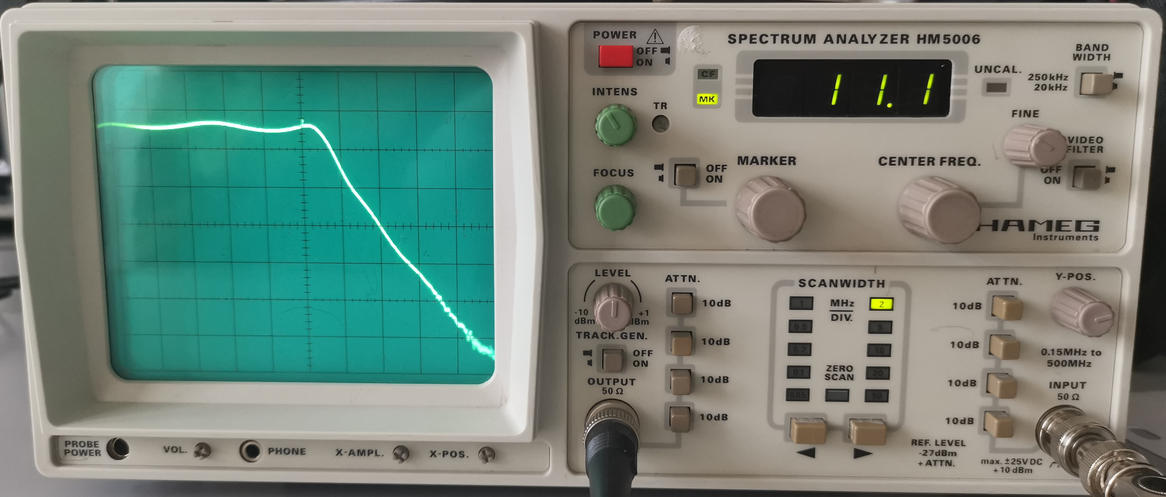
\includegraphics[scale=0.4,keepaspectratio]{img_spectre/analys_spec_bas.PNG}
    \centering
    \caption{Analyseur spectral filtre passe-bas}
\end{figure}
\FloatBarrier

Nous constatons que la fréquence de coupure est très proche de 11.1MHz, ce qui semble conforme au cahier des charges, car il n'y a pas de spécifications sur la stop-band.  

\newpage
\subsubsection{Montage passe-bande de Chebyshev d’ordre 8:} 

\begin{figure}[!htbp]
    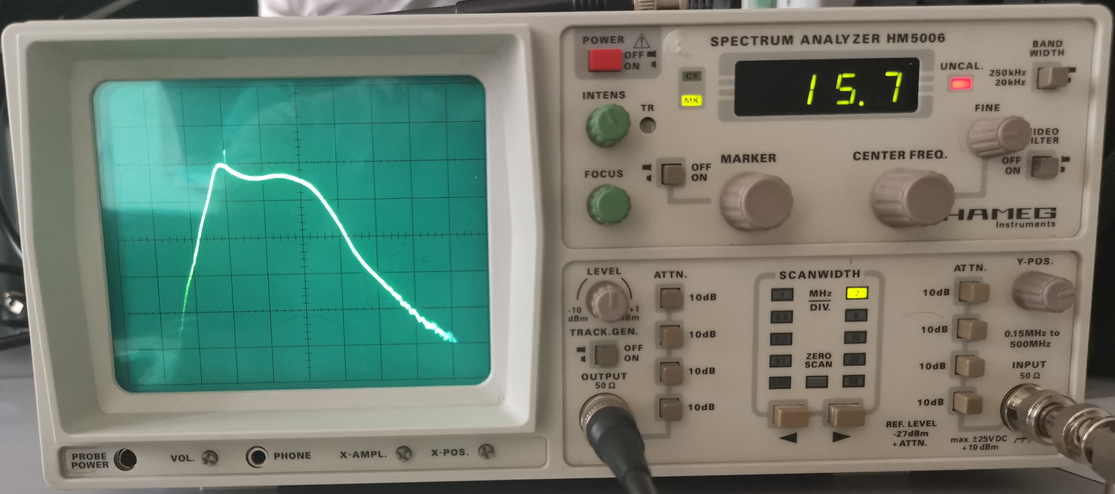
\includegraphics[scale=0.4,keepaspectratio]{img_spectre/analys_spec_bande.PNG}
    \centering
    \caption{Analyseur spectral filtre passe-bande}
\end{figure}
\FloatBarrier

Nous constatons que la fréquence centrale est très proche de 15.7MHz, néanmoins l'atténuation dans la bande passante semble dépasser les contraintes du cahier des charges.

\subsubsection{Montage passe-bas elliptique d'ordre 4:} 

\begin{figure}[!htbp]
    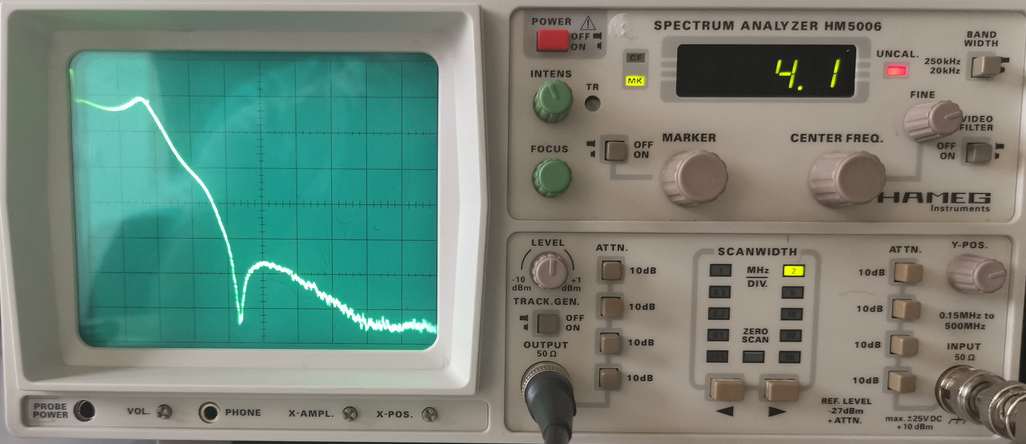
\includegraphics[scale=0.4,keepaspectratio]{img_spectre/analys_spec_elliptique.PNG}
    \centering
    \caption{Analyseur spectral filtre passe-bas elliptique}
\end{figure}
\FloatBarrier


Il s'agit ici du filtre elliptique ayant une fréquence de coupure relativement proche de 4.1MHz. La forme semble bien être celui d'un filtre elliptique typique.

\newpage
D'une manière générale, les courbes obtenues via l'analyseur de spectre coïncident relativement bien au cahier des charges des fonctions de filtrage.
\\
Cependant, il est important de souligner l'une des raisons majeures de leurs erreurs relatives.
En effet, les capacités, inductances et résistances n'auront jamais les mêmes valeurs que ceux obtenus avec les coefficients $g_i$, c'est pour cela qu'il est important de vérifier dans un second temps leurs fiabilités avec les valeurs des composants normalisés (imposé dans le marché). 

\subsection{Comparaison entre le passe-bas et l'elliptique : } 

Nous allons relever du mieux possible les gains à partir de l'analyseur afin de comparer les deux filtres.

Grâce à Excel, nous obtenons les deux courbes suivantes : 

\begin{figure}[!htbp]
    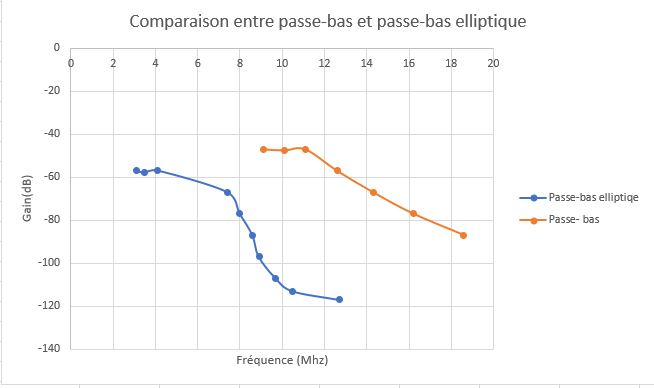
\includegraphics[scale=0.75,keepaspectratio]{img/comparaison.JPG}
    \centering
    \caption{Comparaison filtre passe-bas Chebyshev d'ordre 6 avec filtre elliptique d'ordre 4}
\end{figure}
\FloatBarrier

La principale différence entre les deux filtres est flagrante, le passe-bas elliptique d'ordre 4 a une pente beaucoup plus forte que celle du filtre passe-bas Chebyshev d'ordre 6.

\subsection{Fonction de filtrage : } 

Puisque l'analyseur de spectre trace les gains à partir de la transmittance du montage, nous ne pouvons pas vraiment les exploiter comme telles pour obtenir leurs fonctions de filtrage.

C'est pour cela que nous pouvons en déduire la méthode de passage à la fonction de filtrage en nous appuyant du schéma donné dans le sujet de TP suivant:

\begin{figure}[!htbp]
    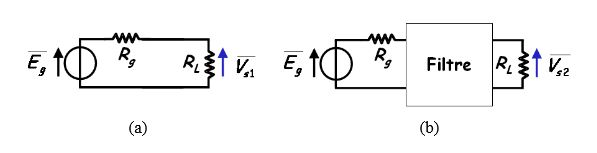
\includegraphics[scale=0.75,keepaspectratio]{img/schema_rappel.JPG}
    \centering
    \caption{Schéma avec et sans filtre}
\end{figure}
\FloatBarrier

Comme la fonction de filtrage est indépendante des impédances de la source et de charge présentes en entrée et en sortie du filtre, nous pourrions utiliser un AOP monté en suiveur afin d'éliminer l'influence de celle-ci.

La fonction de filtrage se définit comme le rapport entre la tension de sortie avec le filtre et la tension de sortie sans le filtre, on peut alors montrer que :

$$ H(w) = \frac{V_s2}{V_s1} \iff H(w) =\frac{V_s2}{\frac{E_g . R_L}{R_L + R_g}} \iff H(w) = \frac{V_s2 . (R_L + R_g)}{E_g . R_L} $$ 














